\documentclass{article}
\usepackage{arxiv}
\usepackage[utf8]{inputenc}
\usepackage[T1]{fontenc}
\usepackage{hyperref}
\usepackage{url}
\usepackage{booktabs}
\usepackage{amsfonts}
\usepackage{amsmath}
\usepackage{graphicx}
\usepackage{float}
\usepackage[french]{babel}
\usepackage{subcaption}

\title{Étude de l'impact des dynamiques non-déterministes sur l'évitement de situations dangereuses en apprentissage par renforcement}

\author{
  Abdelkarim Mouachiq \\
  Université Laval \\
  \texttt{abdelkarim.mouachiq.1@ulaval.ca} \\
  \And
  Saad ElGhissassi \\
  Université Laval \\
  \texttt{saad.elghissassi.1@ulaval.ca} \\
}

\begin{document}
\maketitle

\section{Cas d'étude}

\subsection{Description des composantes de l'environnement}

L'environnement Frozen Lake (v1) de la librairie Gymnasium~\cite{towers2024gymnasium} modélise un lac gelé que l'agent doit traverser pour atteindre un objectif tout en évitant des trous. Chaque cellule de la grille est de l'un des types suivants~: départ (\texttt{S}), surface gelée (\texttt{F}), trou (\texttt{H}) ou objectif (\texttt{G}). L'agent dispose de quatre actions~: gauche, bas, droite et haut. En mode glissant, chaque action a une probabilité de $\frac{1}{3}$ de produire le déplacement voulu et $\frac{1}{3}$ pour chacune des deux directions perpendiculaires. L'agent reçoit une récompense de $+1$ uniquement s'il atteint l'objectif.

\subsection{Ajustement de la difficulté}

Trois paramètres permettent d'ajuster la difficulté~:
\begin{itemize}
    \item \textbf{Stochasticité~:} le paramètre de glissement contrôle si les transitions sont déterministes ou stochastiques, rendant l'évitement des trous plus imprévisible.
    \item \textbf{Nombre de trous~:} une proportion élevée de trous réduit les chemins sûrs disponibles.
    \item \textbf{Positionnement des trous~:} des trous près du chemin optimal forcent l'agent dans des corridors étroits, augmentant le risque de chute.
\end{itemize}

\subsection{Description des cas d'étude}

Nous proposons trois cas d'étude en mode stochastique (surface glissante)~:

\textbf{Cas 1~: Simple (4$\times$4, 1 trou, 6.25\% de danger).}
Grille de 16 cases avec un unique trou placé en position (1,1), adjacent au départ.

\textbf{Cas 2~: Modéré (8$\times$8, 10 trous, 15.6\% de danger).}
Grille de 64 cases. Les deux premières lignes sont libres de trous, tandis que les trous sont concentrés dans les lignes 3 à 8, formant des corridors de passage étroits en bas de la grille.

\textbf{Cas 3~: Difficile (8$\times$8, 17 trous, 26.6\% de danger).}
Grille de 64 cases avec des trous répartis sur l'ensemble de la grille, ne laissant que des passages d'une case de large entre le départ et l'objectif. La figure~\ref{fig:study_cases} illustre les trois configurations.

\begin{figure}[H]
    \centering
    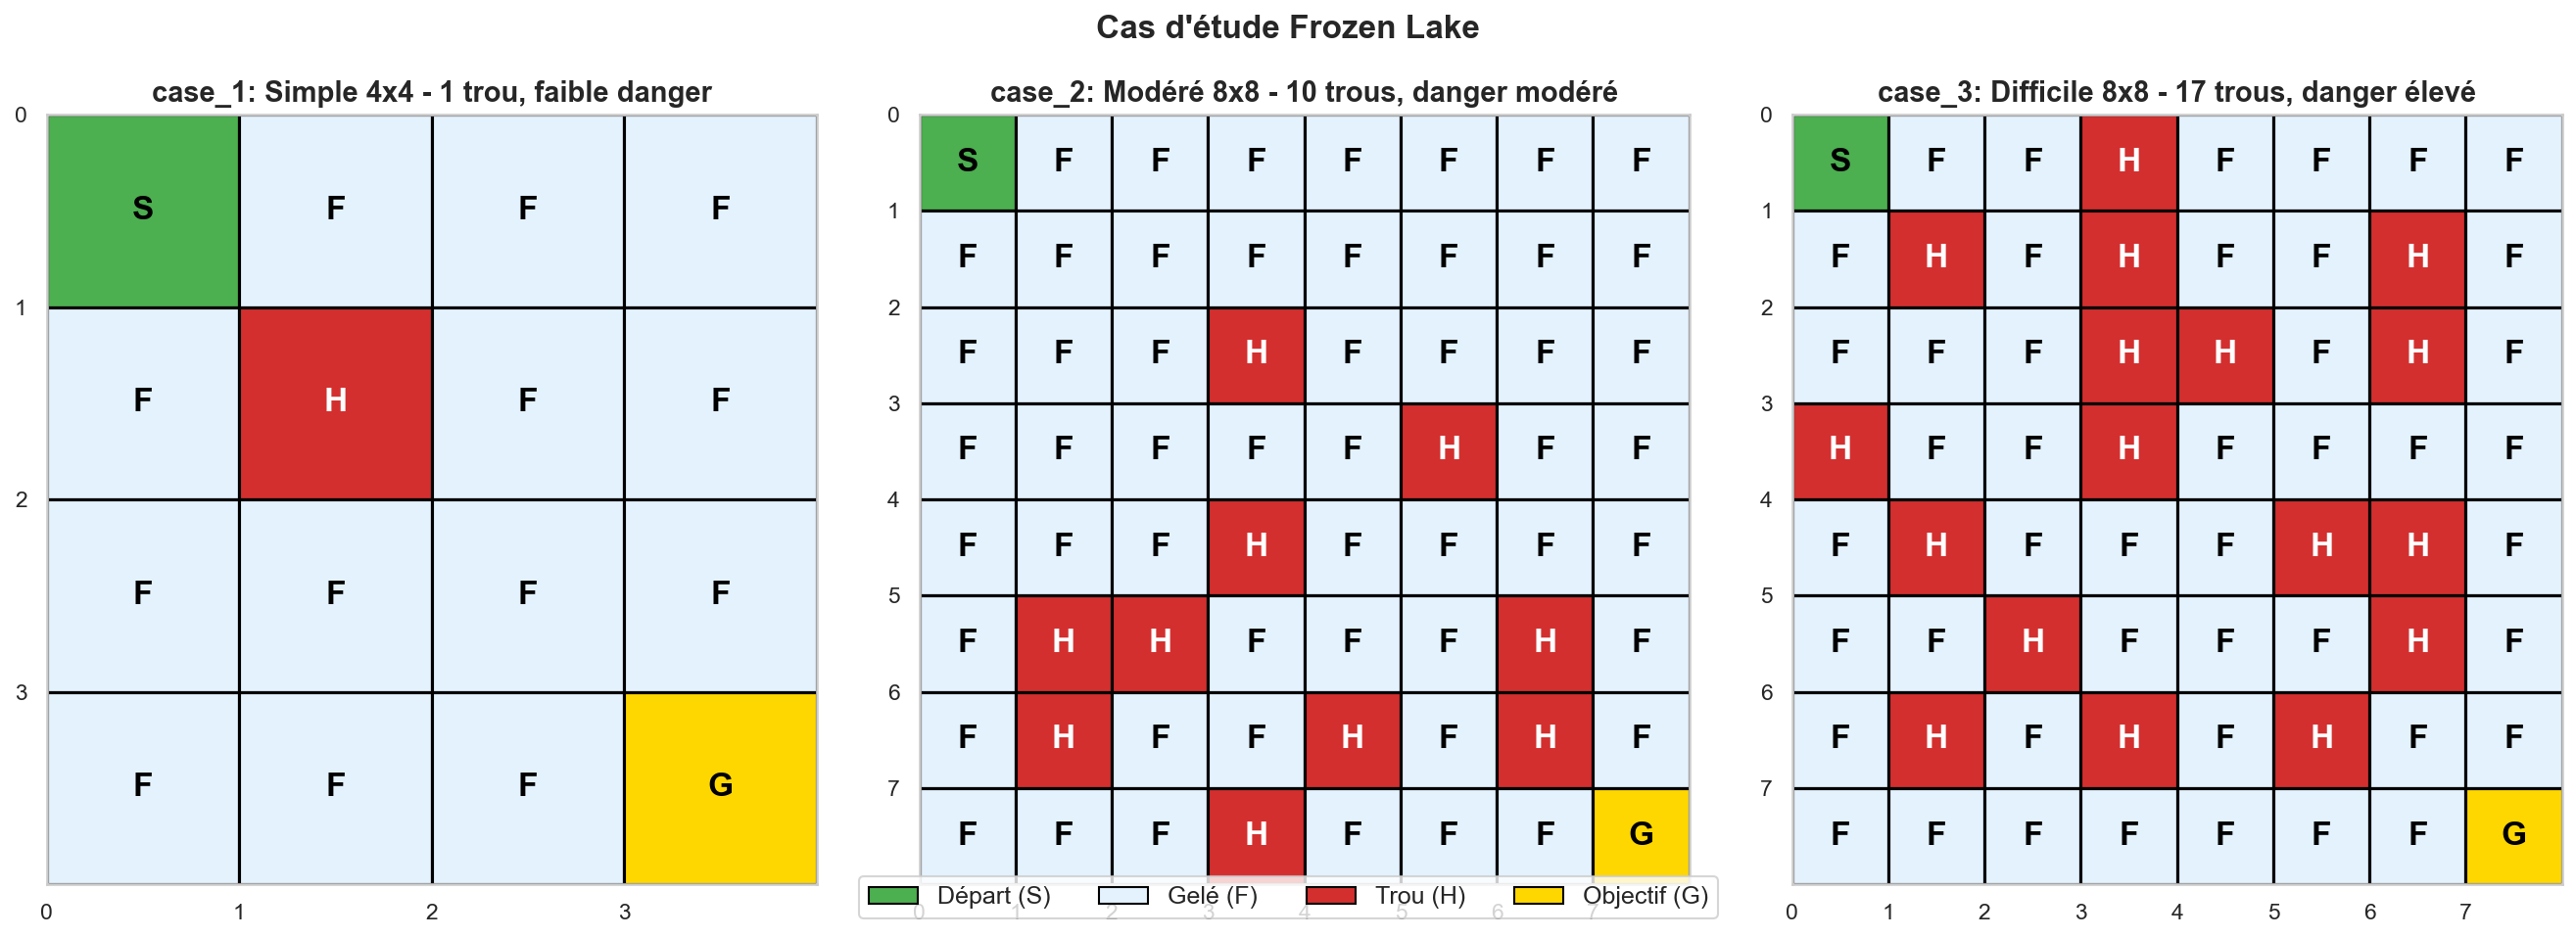
\includegraphics[width=\textwidth]{figures/study_cases.png}
    \caption{Configurations des trois cas d'étude. Vert~: départ, bleu~: gelé, rouge~: trou, jaune~: objectif.}
    \label{fig:study_cases}
\end{figure}

\subsection{Motivation des cas d'étude}

Le nombre et le positionnement des trous dans chaque grille ont été choisis pour construire un gradient de difficulté croissant, permettant d'observer à quel seuil de danger les stratégies classiques cessent de fonctionner.

Le \textbf{cas 1} ne contient qu'un seul trou afin d'isoler l'effet de la stochasticité~: avec une densité de danger de seulement 6.25\%, la difficulté provient uniquement du glissement ($\frac{1}{3}$ de déviation) et non des obstacles. Ce cas sert de référence où toute stratégie raisonnable devrait converger.

Pour le \textbf{cas 2}, le passage à une grille 8$\times$8 augmente l'espace d'états de 16 à 64. Les 10 trous (15.6\%) sont concentrés dans la moitié inférieure, créant une zone haute dégagée et une zone basse avec des corridors étroits où le glissement stochastique augmente le risque de chute.

Le \textbf{cas 3} porte la densité à 17 trous (26.6\%), soit le maximum que la grille peut contenir tout en garantissant un chemin de \texttt{S} vers \texttt{G}. Au-delà (ex.~20 trous, 31\%), aucun chemin viable ne subsiste. La grille reste solvable en mode déterministe, donc tout échec en mode stochastique est attribuable à la combinaison glissement--densité. Ce cas constitue le scénario le plus exigeant pour évaluer le besoin de RL sécuritaire.

\section{Stratégies considérées}

Nous comparons deux stratégies de référence qui ne disposent pas de mécanismes pour gérer les situations dangereuses~\cite{garcia2015comprehensive}.

\subsection{DQN (Deep Q-Network)}

DQN~\cite{mnih2015human} approxime la fonction $Q(s,a)$ via un réseau de neurones profond. Il utilise un tampon de rejeu d'expérience pour casser les corrélations temporelles et un réseau cible mis à jour périodiquement pour stabiliser l'apprentissage. La politique $\varepsilon$-gloutonne choisit l'action de plus haute valeur Q avec probabilité $1{-}\varepsilon$ et une action aléatoire sinon.

\textbf{Motivation~:} algorithme fondamental basé sur l'approximation de la fonction de valeur, dont l'exploration $\varepsilon$-gloutonne ne tient pas compte du danger, permettant d'observer les limitations des approches classiques.

\subsection{PPO (Proximal Policy Optimization)}

PPO~\cite{schulman2017proximal} optimise directement la politique $\pi_\theta(a|s)$ via une fonction objectif avec troncature empêchant les mises à jour trop importantes. Il utilise l'estimateur d'avantage généralisé (EAG) pour réduire la variance des gradients.

\textbf{Motivation~:} contrairement à DQN qui apprend une fonction de valeur, PPO est une méthode de gradient de politique. Ce choix permet de comparer deux familles d'algorithmes fondamentalement différentes~: méthodes basées sur la valeur (DQN) et méthodes basées sur la politique (PPO). PPO a été préféré à A2C et SAC pour sa stabilité reconnue et sa large adoption, tout en restant dépourvu de mécanisme d'évitement des états dangereux.

\section{Méthodologie expérimentale}

\subsection{Hyper-paramètres}

Les deux stratégies sont implémentées via Stable-Baselines3~\cite{raffin2021stable}. Les hyper-paramètres ont été déterminés par recherche sur grille sur le cas 1, puis ajustés pour les cas plus complexes.

\begin{table}[H]
\centering
\caption{Hyper-paramètres de DQN et PPO pour les trois cas d'étude.}
\label{tab:params}
\small
\begin{tabular}{lcccccc}
\toprule
 & \multicolumn{3}{c}{\textbf{DQN}} & \multicolumn{3}{c}{\textbf{PPO}} \\
\cmidrule(lr){2-4} \cmidrule(lr){5-7}
Paramètre & C1 & C2 & C3 & C1 & C2 & C3 \\
\midrule
Taux d'apprentissage & $10^{-3}$ & $5{\times}10^{-4}$ & $5{\times}10^{-4}$ & $3{\times}10^{-4}$ & $3{\times}10^{-4}$ & $3{\times}10^{-4}$ \\
$\gamma$ & 0.99 & 0.99 & 0.99 & 0.99 & 0.99 & 0.99 \\
Taille du lot & 64 & 128 & 128 & 64 & 128 & 128 \\
$\varepsilon$ final / Coeff. entropie & 0.05 & 0.05 & 0.05 & 0.01 & 0.01 & 0.02 \\
Pas de temps totaux & 50k & 100k & 150k & 50k & 100k & 150k \\
\bottomrule
\end{tabular}
\end{table}

\subsection{Indicateurs de performance}

L'objectif ne se limitant pas à maximiser la récompense finale, nous utilisons~:
\begin{itemize}
    \item \textbf{Taux de succès~:} proportion d'épisodes où l'agent atteint l'objectif.
    \item \textbf{Taux de chutes (évaluation)~:} proportion d'épisodes où l'agent tombe dans un trou.
    \item \textbf{Taux de chutes cumulatif (entraînement)~:} ratio chutes/épisodes \textit{durant} l'apprentissage, quantifiant le coût en situations dangereuses.
    \item \textbf{Récompense moyenne~:} récompense moyenne sur les épisodes d'évaluation.
\end{itemize}

\subsection{Paramètres expérimentaux}

Chaque expérience est répétée avec 5 graines aléatoires (42, 123, 456, 789, 1024) pour obtenir des intervalles de confiance. L'évaluation est effectuée périodiquement (toutes les 1\,000 à 3\,000 étapes selon le cas) sur 20 épisodes en mode déterministe. Les épisodes sont limités à 100 pas (cas 1) et 200 pas (cas 2-3). Le code source est structuré en modules (environnement, entraînement, expériences, visualisation) avec un fichier \texttt{requirements.txt} pour la reproductibilité~: \url{https://github.com/Karimartcode/Frozen_Lake_RL}.

\section{Résultats}

\subsection{Performance finale}

Le tableau~\ref{tab:baseline_results} présente les performances finales.

\begin{table}[H]
\centering
\caption{Comparaison des performances des stratégies de référence (moyenne $\pm$ écart-type, 5 graines).}
\label{tab:baseline_results}
\small
\begin{tabular}{llccc}
\toprule
Stratégie & Cas & Taux de succès & Taux de chutes & Récompense moy. \\
\midrule
DQN & Cas 1 & $99.0 \pm 2.0\%$ & $0.0 \pm 0.0\%$ & $0.990 \pm 0.020$ \\
DQN & Cas 2 & $41.0 \pm 18.5\%$ & $2.0 \pm 4.0\%$ & $0.410 \pm 0.185$ \\
DQN & Cas 3 & $0.0 \pm 0.0\%$ & $99.0 \pm 2.0\%$ & $0.000 \pm 0.000$ \\
\midrule
PPO & Cas 1 & $100.0 \pm 0.0\%$ & $0.0 \pm 0.0\%$ & $1.000 \pm 0.000$ \\
PPO & Cas 2 & $27.0 \pm 24.8\%$ & $14.0 \pm 17.4\%$ & $0.270 \pm 0.248$ \\
PPO & Cas 3 & $0.0 \pm 0.0\%$ & $100.0 \pm 0.0\%$ & $0.000 \pm 0.000$ \\
\bottomrule
\end{tabular}
\end{table}


Sur le cas 1, les deux stratégies atteignent $\sim$100\% de succès. Sur le cas 2, les performances se dégradent nettement (DQN~: 41\%, PPO~: 27\%), avec une grande variance entre les graines~: certaines convergent vers un chemin viable tandis que d'autres restent piégées. Sur le cas 3, les deux stratégies échouent complètement (0\% de succès, 100\% de chutes), confirmant que la combinaison densité--glissement rend l'environnement insoluble sans mécanisme de sécurité.

\subsection{Courbes d'apprentissage}
La figure~\ref{fig:success_rate} présente l'évolution du taux de succès au cours de l'entraînement. Sur le cas 1, les deux stratégies convergent rapidement (avant 20\,000 pas). Sur le cas 2, les courbes montrent une forte instabilité~: DQN oscille entre 0\% et 80\% selon les évaluations, tandis que PPO peine à dépasser 40\%. Le cas 3 confirme l'absence totale de convergence.
\begin{figure}[H]
    \centering
    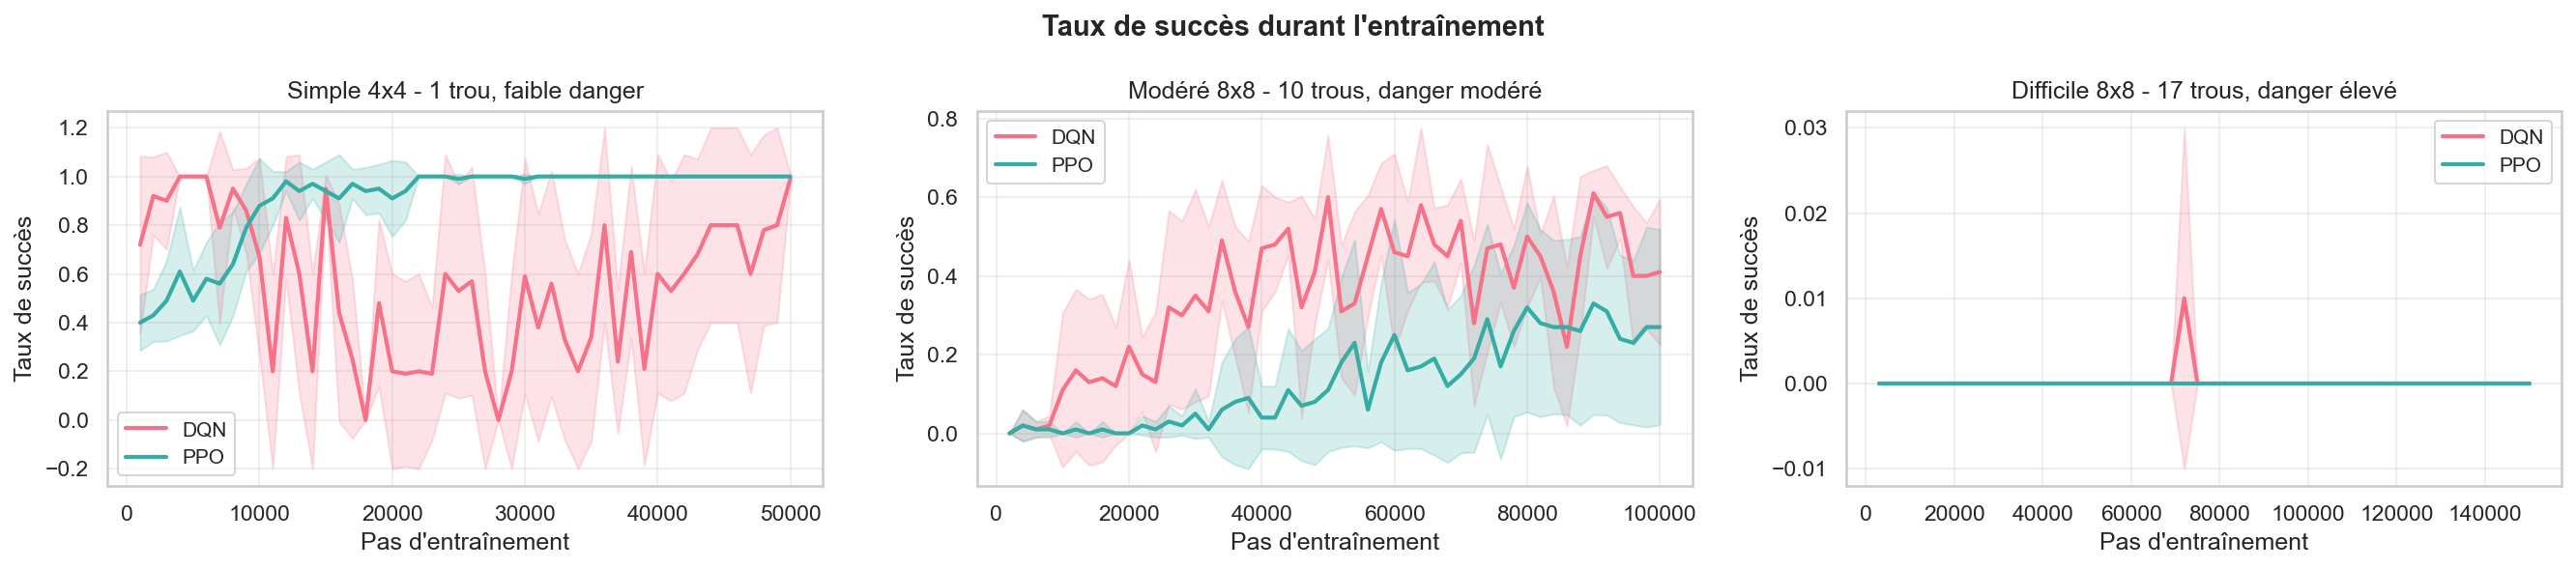
\includegraphics[width=\textwidth]{figures/success_rate.png}
    \caption{Taux de succès durant l'entraînement (moyenne $\pm$ écart-type, 5 graines).}
    \label{fig:success_rate}
\end{figure}
La figure~\ref{fig:train_hole_rate} montre que même sur le cas 1, où la politique finale atteint $\sim$100\% de succès, le taux de chutes durant l'apprentissage reste élevé ($\sim$50\%). L'agent tombe dans un trou environ une fois sur deux pendant qu'il apprend, ce qui serait inacceptable dans un contexte réel où chaque chute a un coût. Cette observation motive directement le recours à des stratégies de RL sécuritaire~\cite{garcia2015comprehensive}.
\begin{figure}[H]
    \centering
    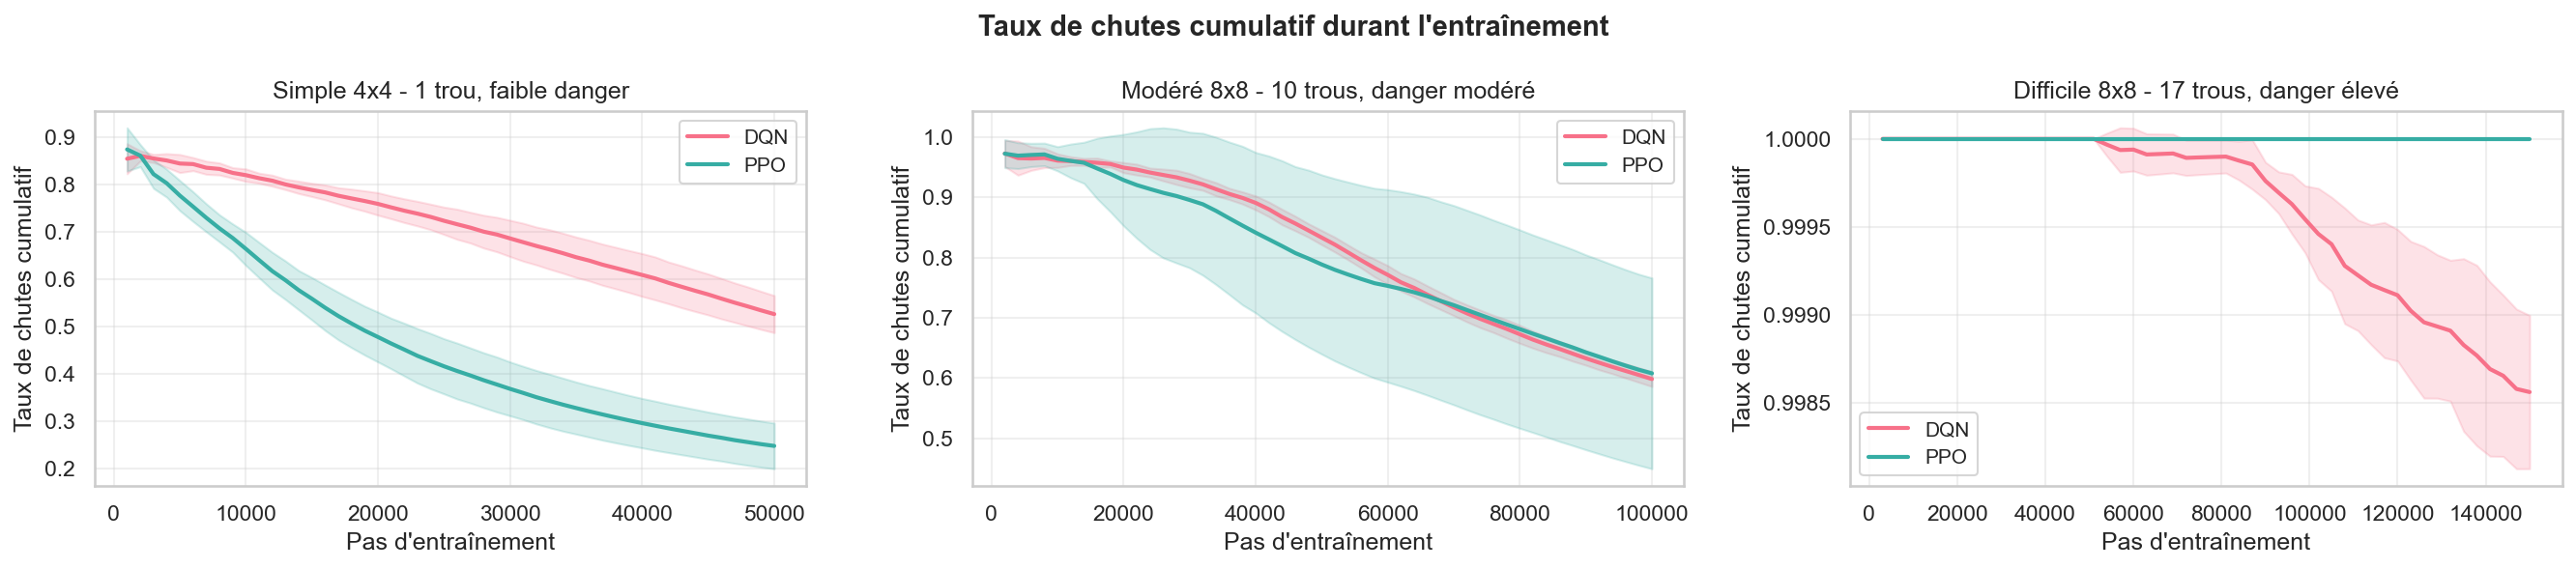
\includegraphics[width=\textwidth]{figures/train_hole_rate.png}
    \caption{Taux de chutes cumulatif durant l'entraînement (moyenne $\pm$ écart-type, 5 graines).}
    \label{fig:train_hole_rate}
\end{figure}
\subsection{Politiques apprises}
La figure~\ref{fig:policies} visualise les politiques apprises sur le cas 1. Les deux stratégies contournent le trou par des directions différentes, illustrant la multiplicité des politiques optimales dans un environnement glissant. Sur les cas 2 et 3, les politiques montrent des actions sous-optimales. Ces résultats guideront notre sélection de stratégies de RL sécuritaire pour le rapport final.
\begin{figure}[H]
    \centering
    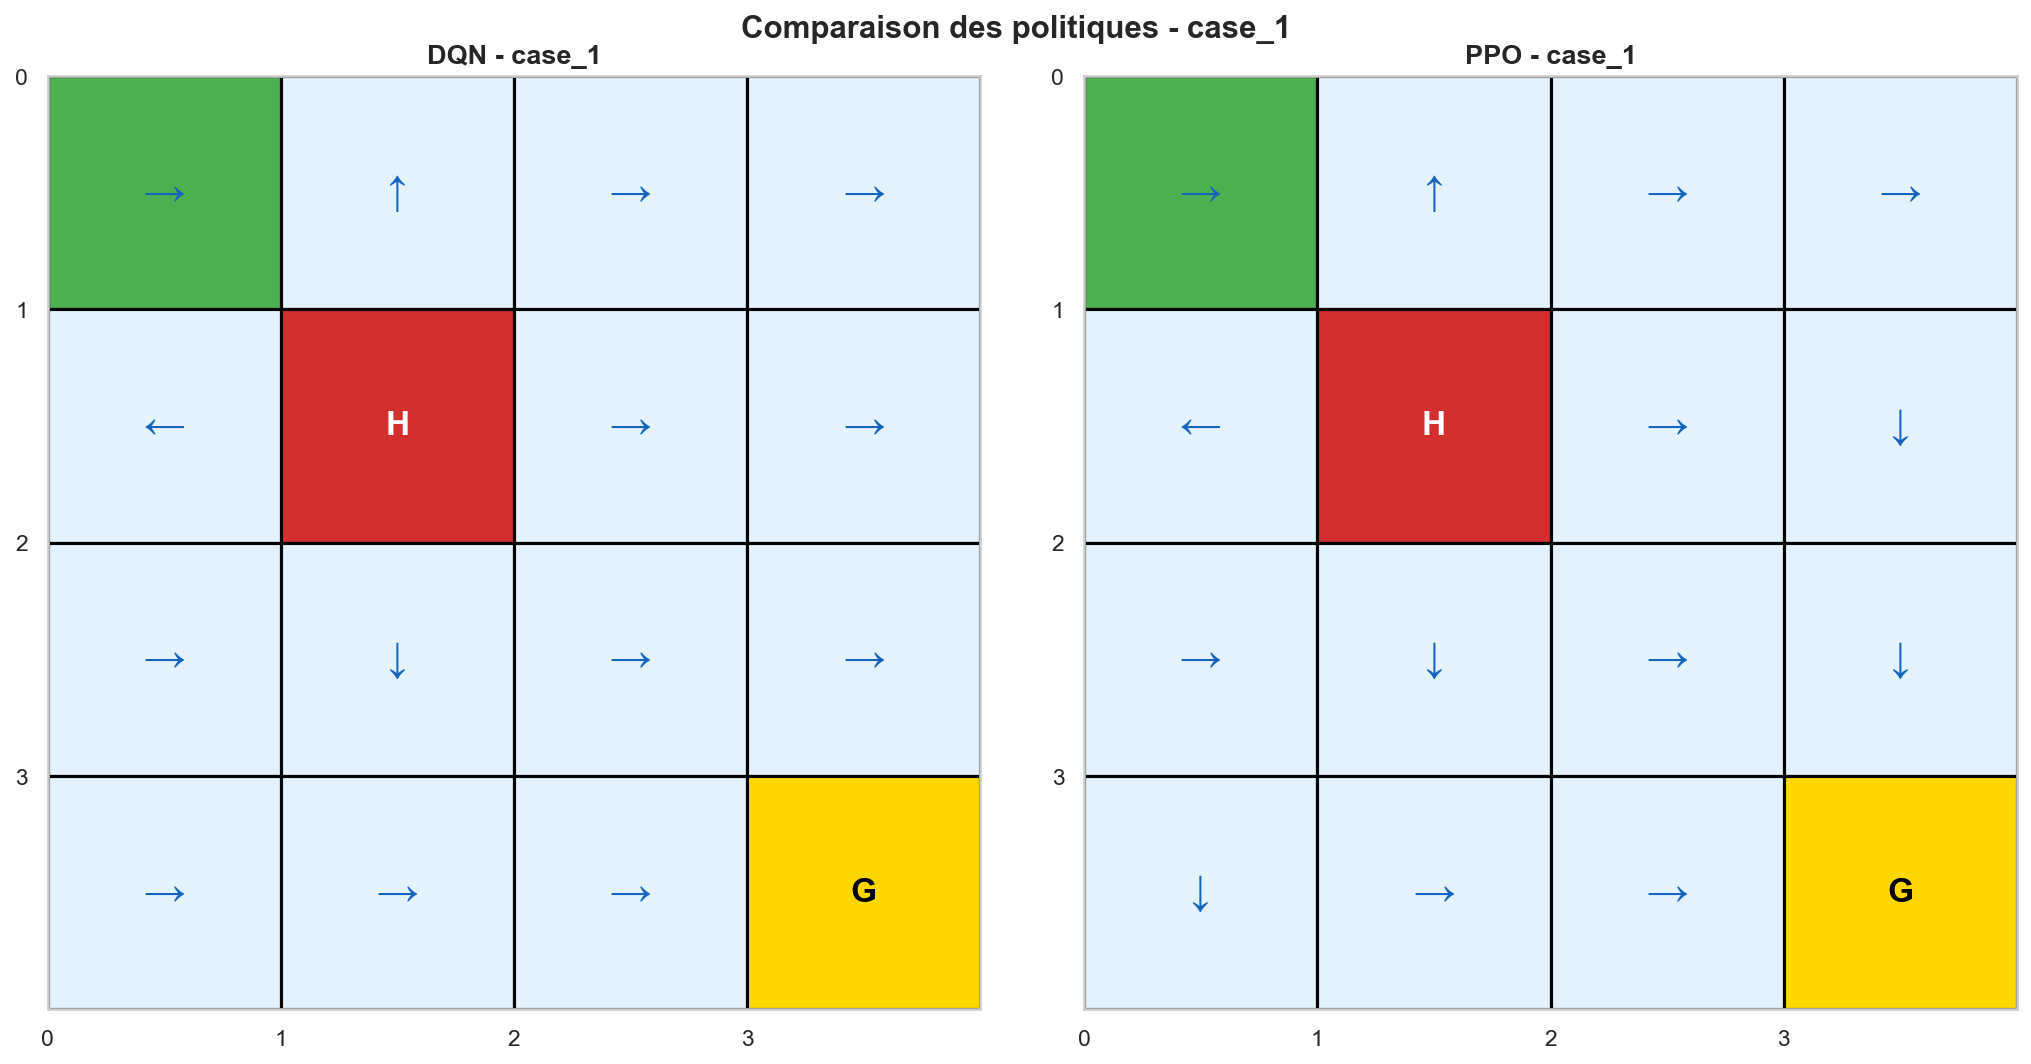
\includegraphics[width=0.5\textwidth]{figures/policy_case_1.png}
    \caption{Politiques apprises par DQN et PPO sur le cas 1.}
    \label{fig:policies}
\end{figure}

\bibliographystyle{plain}
\bibliography{references}

\end{document}
